\chapter{Autonomous Navigation Method}
\label{mainone}
%\textit{
%DELETEME: In this chapter you start addressing your actual problem. Therefore, it makes often sense to make a detailed problem analysis first (if not done in introduction). You should be sure about what to do and how. As writtin in the background part, it might also make sense to include complex background information or papers you are basing on in this analysis. If you are solving a software problem, you should follow the state of the art of software development which basically includes: problem analysis, design, implementation, testing, and deployment. Maintenance is often also described but I believe this will not be required for most theses. Code should be placed in the appendix unless it is solving an essential aspect of your work.
%}


This chapter presents 
the autonomous drone racing method of Kaufmann et al. \cite{Kaufmann2018},
which is used as a baseline for the experiments of this thesis.
The first section introduces the three reference systems 
and their transformations applied by the modules of the method.
The second section presents the ANN module of this thesis,
which has the function of making navigation decisions 
based on the RGB images from the drone's onboard camera.
The ANN module comprising the CNN, CAT, FC, GRU and HEAD submodules
is a modularized version of the ANN of the baseline work
that additionally integrates the CAT submodule,
which extends the decision-making basis with the optional inputs
(i.e., the time steps of the images and 
the estimates from the drone's onboard IMU)
and the GRU submodule,
which extends the decision-making capabilities with temporal comprehension.
The third section presents the planning module of the method,
which has the function of computing local trajectories 
based on the navigation decisions made by
the ANN module or, in the imitation learning process, the expert system.
The fourth section presents the control stack of the method,
which has the function to compute the drone's motor inputs 
to track the local trajectories computed by the planning module.
The fifth section presents the expert system of the method,
which in the rollouts of the imitation learning process,
intervenes and generates a training sample
whenever the ANN module makes a poor navigation decision.



\section{Reference Systems}
In this thesis, the coordinates of a point 
$\pos[]{}{}{}{}$
relate to either the global, the local or the image reference system
\begin{equation}
    \pos[]{}{}{\grs}{} = \begin{bmatrix}
        \x[]{}{}{\grs}{} \\ \y[]{}{}{\grs}{} \\ \z[]{}{}{\grs}{}
    \end{bmatrix} \in \mathbb{R}^3
    ,\quad 
    \pos[]{}{}{\lrs}{} = \begin{bmatrix}
        \x[]{}{}{\lrs}{} \\ \y[]{}{}{\lrs}{} \\ \z[]{}{}{\lrs}{}
    \end{bmatrix} \in \mathbb{R}^3
    ,\quad 
    \pos[]{}{}{\irs}{} = \begin{bmatrix}
        \x[]{}{}{\irs}{} \\ \y[]{}{}{\irs}{}
    \end{bmatrix} \in \left[\text -1, 1\right]^2.
\end{equation}


The 3D global reference system
is fixed to an arbitrary point on earth
and is hence quasi inertial.
It is spanned by the orthonormal basis,
which, related to the global reference system,
equates to the standard basis of $\mathbb{R}^3$
\begin{equation}
    \left\{
        \unitvec[]{\text G}{x}{}{},
        \unitvec[]{\text G}{y}{}{},
        \unitvec[]{\text G}{z}{}{}
    \right\}
    \quad \text{with} \quad 
    \unitvec[]{\text G}{x}{\grs}{} = \begin{bmatrix} 1 \\ 0 \\ 0 \end{bmatrix},\ 
    \unitvec[]{\text G}{y}{\grs}{} = \begin{bmatrix} 0 \\ 1 \\ 0 \end{bmatrix},\ 
    \unitvec[]{\text G}{z}{\grs}{} = \begin{bmatrix} 0 \\ 0 \\ 1 \end{bmatrix}.
\end{equation}


The local reference system (see fig. \ref{fig:local_reference_system}) is fixed on the moving drone.
It is spanned by the orthonormal basis,
whose origin is located at the optical center of the drone's onboard camera
\begin{equation}
    \left\{
        \unitvec[]{\text L}{x}{}{},
        \unitvec[]{\text L}{y}{}{},
        \unitvec[]{\text L}{z}{}{}
    \right\}
    \quad \text{with} \quad 
    \unitvec[]{\text L}{x}{\lrs}{} = \begin{bmatrix} 1 \\ 0 \\ 0 \end{bmatrix},\ 
    \unitvec[]{\text L}{y}{\lrs}{} = \begin{bmatrix} 0 \\ 1 \\ 0 \end{bmatrix},\ 
    \unitvec[]{\text L}{z}{\lrs}{} = \begin{bmatrix} 0 \\ 0 \\ 1 \end{bmatrix}.
\end{equation}
The unit vector 
$\unitvec[]{\text L}{x}{}{}$ 
points along the optical axis of the camera
in the flight direction of the drone.
The unit vector
$\unitvec[]{\text L}{z}{}{}$ 
points in the direction of the forces generated by the drone's rotors
and is parallel to the vertical axis of the image plane of the drone's onboard camera.
The unit vector 
$\unitvec[]{\text L}{y}{}{}$ 
points to the left of the drone
and parallels the horizontal axis of the image plane.






The image reference system (see fig. \ref{fig:image_reference_system}) 
is superimposed on the images of the drone's onboard camera.
This 2-dimensional system is spanned by the orthonormal basis
\begin{equation}
    \left\{
        \unitvec[]{\text I}{x}{}{},
        \unitvec[]{\text I}{y}{}{}
    \right\}
    \quad \text{with} \quad 
    \unitvec[]{\text I}{x}{\irs}{} = \begin{bmatrix} 1 \\ 0 \end{bmatrix},\ 
    \unitvec[]{\text I}{y}{\irs}{} = \begin{bmatrix} 0 \\ 1 \end{bmatrix}.
\end{equation}
The origin of the image reference system 
is located at the center of the image plane.
The unit vector 
$\unitvec[]{\text I}{x}{}{}$  
points rightwards along the vertical axis of the image plane.
The unit vector 
$\unitvec[]{\text I}{y}{}{}$  
points upwards along the horizontal axis of the image plane.
A point on the image plane 
is bounded by the left and right
$ -1 \le \x[]{}{}{\irs}{} \le 1 $
as well as the lower and upper
$ -1 \le \y[]{}{}{\irs}{} \le 1 $
border of the image plane.
%The global reference system 
%is only referred to 
%by the expert system (see section)
%which makes navigation decisions based on globally consistent information
%when generating training data for the ANN module.
%The autonomous navigation method, 
%with the fully trained ANN module making the navigation decisions,
%exclusively resorts to data from onboard sensors,
%which is relative to the drone and its onboard camera.
%The method, therefore, operates only within the local and image reference system.
\begin{figure}[h]
    \centering
    \subfloat[
        Local reference system
    ]{
        \label{fig:local_reference_system}
        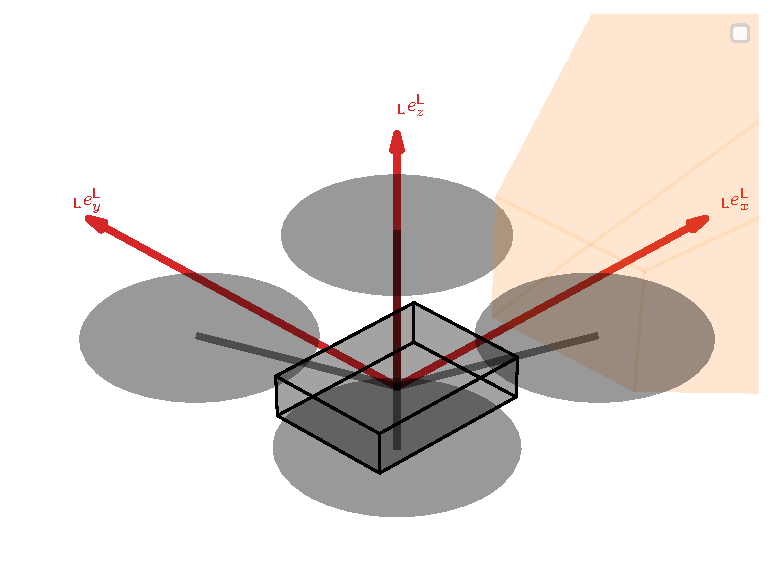
\includegraphics[width=0.441\textwidth]{own/local_reference_system.pdf}
    }                
    \subfloat[
        Image reference system
    ]{
        \label{fig:image_reference_system}
        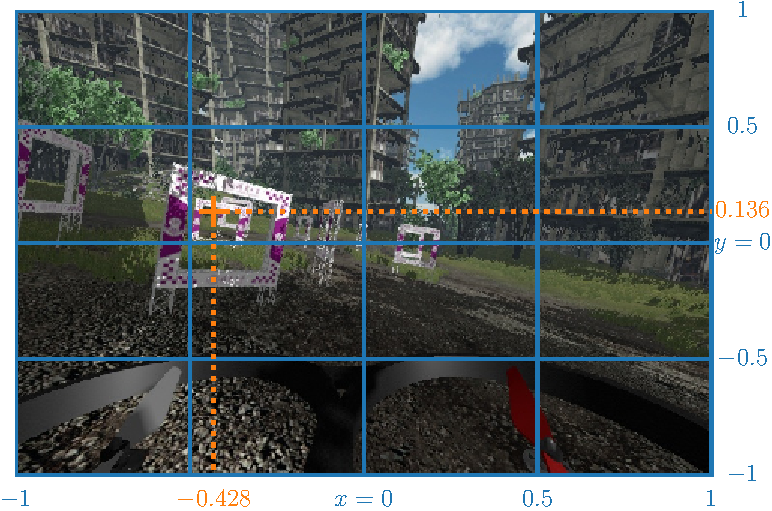
\includegraphics[width=0.5\textwidth]{own/image_reference_system.pdf}
    }
    \caption[
        Local and image reference system
    ]{
        The local and the image reference system. 
        The local reference system (red) is aligned with the drone's onboard camera. 
        The image reference system (blue) is superimposed on the images from the onboard camera.
        The pictured, exemplary waypoint
        $\pos[]{\wayp}{}{\irs}{} = \begin{bmatrix} -0.428 & 0.136 \end{bmatrix}^T$
        (orange) with respect to the image reference system
        is part of the label for the underlying image.
        \label{fig:local_and_image_reference_system}
    }
\end{figure}
%https://www.researchgate.net/figure/Pin-hole-camera-model-terminology-The-optical-center-pinhole-is-placed-at-the-origin_fig10_317498100





\paragraph*{Global-local Transformations} $\ $\\
The drone's position
$\pos[]{\drone}{}{\grs}{}$
and quaternion orientation
$\quat[]{\drone}{}{\grs}{}$
with respect to the global reference system
are the parameters that determine the bidirectional transformation
between the global and the local reference system.
The following bases on quaternion mathematics,
for which one can consult, e.g., \cite{Parent}.
A point given in the coordinates of the global reference system
can be expressed in the coordinates of the local reference system
with the transformation
\begin{align} \label{equ:global_to_local_transformation}
    \trafo[]{}{\lrs\grs}{}{}
    :\ 
    \mathbb{R}^3 \rightarrow \mathbb{R}^3
    ; \quad
    \pos[]{}{}{\grs}{} \mapsto \pos[]{}{}{\lrs}{}
    =
    %\begin{cases}
        \mathcal{P} \left[
            \mathrm{inv} \left( \quat[]{\drone}{}{\grs}{} \right)
            *
            \mathcal{Q} \left( \pos[]{}{}{\grs}{} - \pos[]{\drone}{}{\grs}{} \right)
            *
            \quat[]{\drone}{}{\grs}{}
        \right], 
        %& \text{if } \quat[]{\drone}{}{\grs}{} \ne \underline 0 \\
        %\pos[]{}{}{\grs}{} - \pos[]{\drone}{}{\grs}{}, 
        %& \text{else}.
    %\end{cases}
\end{align}
Reversely, a point given in the coordinates of the local reference system
can be expressed in the coordinates of the global reference system
with the transformation
\begin{align} \label{eq:local_to_global_transformation}
    \trafo[]{}{\grs\lrs}{}{}
    :\ 
    \mathbb{R}^3 \rightarrow \mathbb{R}^3
    ; \quad
    \pos[]{}{}{\lrs}{} \mapsto \pos[]{}{}{\grs}{}
    =
    %\begin{cases}
        \mathcal{P} \left[
            \quat[]{\drone}{}{\grs}{}
            *
            \mathcal{Q} \left( \pos[]{}{}{\lrs}{} \right)
            *
            \mathrm{inv} \left( \quat[]{\drone}{}{\grs}{} \right)
        \right] + \pos[]{\drone}{}{\grs}{}. 
        %& \text{if } \quat[]{\drone}{}{\grs}{} \ne \underline 0 \\
        %\pos[]{}{}{\lrs}{} + \pos[]{\drone}{}{\grs}{}, 
        %& \text{else}.
    %\end{cases}
\end{align}
In the two above transformations,
the mapping $\mathcal{Q}$
of a point to its quaternion representation 
and the reverse mapping $\mathcal{P}$ 
of a quaternion representation to its point  
are given by
\begin{align}
    \mathcal{Q}
    :\ 
    & \mathbb{R}^3 \rightarrow \mathbb{R}^4
    ;\
    \pos[]{}{}{}{} = \begin{bmatrix} \x[]{}{}{}{} \\ \y[]{}{}{}{} \\ \z[]{}{}{}{} \end{bmatrix} 
    \mapsto
    \quat[]{}{}{}{} = \begin{bmatrix} w \\ \underline p \end{bmatrix} 
    \text{ with } w = 0
    \nonumber \\
    \mathcal{P}
    :\ 
    &\mathbb{R}^4 \rightarrow \mathbb{R}^3
    ;\
    \quat[]{}{}{}{} = \begin{bmatrix} w \\ \underline p \end{bmatrix} 
    \mapsto
    \pos[]{}{}{}{} = \begin{bmatrix} \x[]{}{}{}{} \\ \y[]{}{}{}{} \\ \z[]{}{}{}{} \end{bmatrix}.
\end{align}
Moreover, the operator $*$ denotes the multiplication of two quaternions, which is given by
\begin{align}
    \quat[]{}{1}{}{} * \quat[]{}{2}{}{}
    = 
    \begin{bmatrix}
        w_1 w_2 - \pos[]{T}{1}{}{} \pos[]{}{2}{}{}\\ 
        w_1 \pos[]{}{2}{}{} + w_2 \pos[]{}{1}{}{} + \pos[]{}{1}{}{} \times \pos[]{}{2}{}{}
    \end{bmatrix}.
\end{align}
Finally, the inversion of a quaternion is given by
\begin{align}
    \mathrm{inv}(\quat[]{}{}{}{}) 
    = 
    \frac{1}{\| \quat[]{}{}{}{} \|_2}
    \begin{bmatrix} w \\ \text - \pos[]{}{}{}{} \end{bmatrix}.
\end{align}
The two above transformations are the inversion of each other.
Therefore, points can be transformed between the global and local reference system
without information loss
\begin{equation}
    \trafo[]{}{\grs\lrs}{}{} \circ \trafo[]{}{\lrs\grs}{}{} 
    \left( \pos[]{}{}{\grs}{} \right)
    =
    \pos[]{}{}{\grs}{}
    ,\quad
    \trafo[]{}{\lrs\grs}{}{} \circ \trafo[]{}{\grs\lrs}{}{} 
    \left( \pos[]{}{}{\lrs}{} \right)
    =
    \pos[]{}{}{\lrs}{}.
\end{equation}
In the above equations, the operator $\circ$ denotes the composition of two functions.



\paragraph*{Local-image Transformation} $\ $\\
The horizontal
$\ang[\user]{\camera}{\text h}{}{}$
and the vertical
$\ang[\user]{\camera}{\text v}{}{}$
angle of view
of the drone's onboard camera
are the parameters 
that determine the bidirectional transformation 
between the local and the image reference system.
A point given in the coordinates of the local reference system
is expressed in the coordinates of the image reference system with the transformation
\begin{align} \label{equ:local_to_image_transformation}
    \trafo[]{}{\irs\lrs}{}{}
    :\ 
    \mathbb{R}^3 \rightarrow \left[ \text{-}1, 1 \right]^2
    ; \quad
    \pos[]{}{}{\lrs}{} \mapsto \pos[]{}{}{\irs}{}
    =
    \begin{bmatrix}
        \maxof{\text -1}{
            \minof{
                \frac{\text -2}{\ang[\user]{\camera}{\text h}{}{}}
                \mathrm{atan2}\left( \y[]{}{}{\lrs}{}, \x[]{}{}{\lrs}{} \right)
            }{1}
        }
        \\
        \maxof{\text -1}{
            \minof{
                \frac{2}{\ang[\user]{\camera}{\text v}{}{}}
            \mathrm{atan2} \left( \z[]{}{}{\lrs}{}, \| \pos[]{}{}{\lrs}{} \|_2 \right)
            }{1}
        }
    \end{bmatrix}
    .
\end{align}
The above transformation
can be interpreted as the projection of a point onto the image plane 
of the drone's onboard camera.
It can be divided into three steps.
First, the vector from the optical center of the camera 
to the point to be transformed
is mapped to its yaw
$\mathrm{atan2}\left( \y[]{}{}{\lrs}{}, \x[]{}{}{\lrs}{} \right)$
and pitch 
$\mathrm{atan2} \left( \z[]{}{}{\lrs}{}, \| \pos[]{}{}{\lrs}{} \|_2 \right)$
angle, both, with respect to the image reference system.
Second these angles are normalized by 
the half of the horizontal 
$\ang[\user]{\camera}{\text h}{}{}$ 
and the half of the vertical
$\ang[\user]{\camera}{\text v}{}{}$
angle of view of the camera, respectively.
Third, these normalized angles are bounded to be in the interval from minus to plus one.
This boundary takes into account 
that an artificial neural network, which inputs images, 
has no basis for predictions 
that relate to objects that are not within the camera's field of view.
As a projection from 3D to 2D, the above transformation is accompanied by information loss
and is hence not bijective.

A point given in the coordinates of the image reference system is expressed
in the coordinates of the local reference system with the reverse transformation
\begin{align} \label{eq:image_to_local_transformation}
    \trafo[]{}{\lrs\irs}{}{}
    &:\ 
    \mathbb{R}_{\ge 0}, \left[ \text{-}1, 1 \right]^2 \rightarrow \mathbb{R}^3
    ; \quad
    d, \pos[]{}{}{\irs}{} \mapsto \pos[]{}{}{\lrs}{}
    =
    d \begin{bmatrix}
        \cos \left( \ang[]{}{y}{\lrs}{} \right) \\
        \cos \left( \ang[]{}{y}{\lrs}{} \right) \\
        \sin \left( \ang[]{}{y}{\lrs}{} \right)
    \end{bmatrix} \odot \begin{bmatrix}
        \cos \left( \ang[]{}{z}{\lrs}{} \right) \\
        \sin \left( \ang[]{}{z}{\lrs}{} \right) \\
        1
    \end{bmatrix}
    \nonumber \\
    & \qquad \text{with} \quad
    \ang[]{}{z}{\lrs}{}
    = 
    \text - \frac{\ang[\user]{\camera}{\text h}{}{}}{2} \cdot \x[]{}{}{\irs}{}
    ,\quad 
    \ang[]{}{y}{\lrs}{}
    = 
    \frac{\ang[\user]{\camera}{\text v}{}{}}{2} \cdot \y[]{}{}{\irs}{}.
\end{align}
In the above transformation,
the operator 
$\odot$ 
denotes the Hadamard product, 
i.e., the element-wise product of two equally dimensioned matrices.
Because the 2D coordinates of the image reference system
can only contain information about the direction of a point,
the above transformation to 3D requires the additional input of a back-projection length $d$.

In contrast to the transformations 
$\trafo[]{}{\lrs\grs}{}{}$
and 
$\trafo[]{}{\grs\lrs}{}{}$
between the global and the local reference system,
the transformations 
$\trafo[]{}{\irs\lrs}{}{}$
and 
$\trafo[]{}{\lrs\irs}{}{}$
between the local and the image reference system
are not invertible.
However, for relevant points
located within the camera's field of view
and a well chosen back-projection length,
it is assumed that the transformations approximately invert each other
\begin{equation}
    \trafo[]{}{\lrs\irs}{}{} \left[
        d, \trafo[]{}{\irs\lrs}{}{} \left( \pos[]{}{}{\lrs}{} \right)
    \right]
    \approx
    \pos[]{}{}{\lrs}{}
    ,\quad
    \trafo[]{}{\irs\lrs}{}{}
    \circ 
    \trafo[]{}{\lrs\irs}{}{} \left(
        d, \pos[]{}{}{\irs}{}
    \right)
    \approx
    \pos[]{}{}{\irs}{}.
\end{equation}





\paragraph*{Global-image Transformation} $\ $\\
The bidirectional transformations of points between the global and the image reference frame
are the compositions of the transformations via the intermittent local reference system
\begin{align} \label{eq:global_image_transformations}
    \trafo[]{}{\irs\grs}{}{}
    &=
    \trafo[]{}{\irs\lrs}{}{} \circ \trafo[]{}{\lrs\grs}{}{}
    :\ 
    \mathbb{R}^3 \rightarrow \left[\text{-} 1, 1\right]^2 
    \nonumber \\
    \trafo[]{}{\grs\irs}{}{}
    &=
    \trafo[]{}{\grs\lrs}{}{} \circ \trafo[]{}{\lrs\irs}{}{}
    :\ 
    \mathbb{R}_{\ge 0}, \left[\text{-} 1, 1\right]^2 \rightarrow \mathbb{R}^3.
\end{align}
Due to the fact that
$\trafo[]{}{\lrs\grs}{}{}$
and
$\trafo[]{}{\grs\lrs}{}{}$
are the inverse of each other
and the assumption that
$\trafo[]{}{\irs\lrs}{}{}$
and
$\trafo[]{}{\lrs\irs}{}{}$
approximately invert each other within a relevant range,
the above compositions are expected to also approximately invert each other within this relevant range
\begin{equation}
    \trafo[]{}{\grs\irs}{}{} \left[
        d, \trafo[]{}{\irs\grs}{}{} \left( \pos[]{}{}{\grs}{} \right)
    \right]
    \approx
    \pos[]{}{}{\grs}{}
    ,\quad
    \trafo[]{}{\irs\grs}{}{}
    \circ 
    \trafo[]{}{\grs\irs}{}{} \left(
        d, \pos[]{}{}{\irs}{}
    \right)
    \approx
    \pos[]{}{}{\irs}{}.
\end{equation}

%\begin{figure}
%    \centering
%    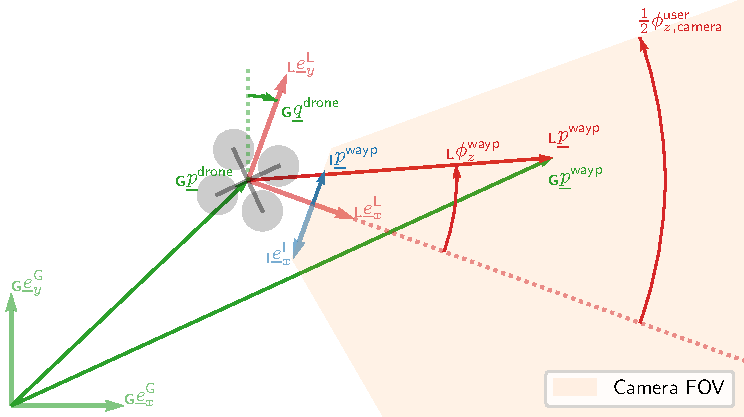
\includegraphics[width=0.9\textwidth]{own/global_via_local_to_image_transformation_2d.pdf}
%    \caption[
%        Schematic 2D depiction
%        of the transformation of the waypoint 
%        from the global via the local to the image reference system.
%    ]{
%        Schematic 2D depiction
%        of the transformation of the waypoint 
%        from the global ${}_\textbf{G}\square$ 
%        via the local ${}_\textbf{L}\square$ 
%        to the image ${}_\textbf{I}\square$ reference system.
%        Unit vectors 
%        $\underline e_\square \in \mathbb{R}^3,\ \left\|\underline e_\square \right\|_2 = 1$ 
%        spanning the individual reference systems,
%        points $\underline p^\square \in \mathbb{R}^3$,
%        quaternions $\underline q^\square \in \mathbb{R}^4$
%        and angles $\phi_\square^\square  \in \mathbb{R}$
%        relative to the global, local or image reference system
%        are colored in green, red or blue, respectively.
%        %Unit vectors are drawn
%        %with a greater linewidth and lower opacity 
%        %than the positions, quaternions and angles.
%        The z unit vectors 
%        ${}_\textbf{G} e^\text{G}_z$
%        and
%        $\ {}_\textbf{L} e^\text{L}_z$ 
%        of the global and local reference system,
%        the y unit vector 
%        ${}_\textbf{I} e^\text{I}_y$ 
%        of the image reference system
%        and the pitch angle 
%        $\phi^\text{user}_{y,\text{camera}}$
%        of view of the camera
%        are not pictured
%        in this 2D representation.
%        %but point in the direction of the reader.
%        The field of view (FOV) of the onboard camera of the drone
%        is marked with a low-opaque orange.
%
%        The global position
%        ${}_\textbf{G}\underline p^\text{drone}$
%        and quaternion orientation
%        ${}_\textbf{G}\underline q^\text{drone}$
%        of the drone,
%        the yaw
%        $\phi^\text{user}_{z,\text{camera}}$
%        and pitch
%        $\phi^\text{user}_{y,\text{camera}}$ 
%        angle of view of the camera
%        as well as the global position of the waypoint
%        ${}_\textbf{G}\underline p^\text{wayp}$
%        are known.
%        First, the local position of the waypoint
%        ${}_\textbf{L}\underline p^\text{wayp}$
%        is computed by applying the transformation
%        $T_\textbf{LG}$
%        (equation \ref{equ:global_to_local_transformation}).
%        Second, 
%        ${}_\textbf{L}\underline p^\text{wayp}$
%        is transformed with 
%        $T_\textbf{IL}$
%        (equation \ref{equ:local_to_image_transformation})
%        yielding 
%        the position of the waypoint
%        ${}_\textbf{I}\underline p^\text{wayp}$ 
%        with respect to the image reference system.
%        $T_\textbf{LG}$ is fully determined by 
%        ${}_\textbf{G}\underline p^\text{drone}$ 
%        and 
%        ${}_\textbf{G}\underline q^\text{drone}$.
%        $T_\textbf{IL}$ is fully determined by
%        $\phi^\text{user}_{z,\text{camera}}$
%        and
%        $\phi^\text{user}_{y,\text{camera}}$.
%        \label{fig:trafo}
%    }
%\end{figure}






%%%%%%%%%%%%%%%%%%%%%%%%%%%%%%%%%%%%%%%%%%%
\section{ANN Module}\label{sec:ann_module}
%
%
\newcommand{\R}[1]{\mathbb{R}^{#1}}
\newcommand{\setR}[1]{\left[#1\right]}

\newcommand{\setOfAllPosInts}{\mathbb{N}_{>0}}
\newcommand{\setOfInts}[1]{\left\{ #1 \right\}}
\newcommand{\placeholder}{\square}
\newcommand{\floor}[1]{\left\lfloor #1 \right\rfloor}
\newcommand{\series}[1]{\left(#1\right)}
\newcommand{\tuple}[1]{\left(#1\right)}
%
\newcommand{\rawRGB}{\img[]{\camera}{}{}{}}
\newcommand{\rawRGBFullInt}{\num[]{\camera}{\mxm}{}{}}
\newcommand{\rawRGBHeight}{\num[]{\camera}{\height}{}{}}
\newcommand{\rawRGBWidth}{\num[]{\camera}{\widthh}{}{}}
\newcommand{\rawRGBTimeStep}{\dur[]{\camera}{}{}{}}
\newcommand{\preprocRGB}[1]{\img[]{\preprocessed}{#1}{}{}}
\newcommand{\IMULinAcc}{\acc[\hat]{\imu}{}{\lrs}{}}
\newcommand{\IMUAngVel}{\angvel[\hat]{\imu}{}{\lrs}{}}
\newcommand{\IMUTimeStep}{\dur[]{\imu}{}{}{}}
\newcommand{\optFeatVec}[1]{\featvec[]{\optional}{#1}{}{}}
\newcommand{\CNNMap}{\Func[\user]{\cnn}{}{}{}}
\newcommand{\CNNNumC}{\num[]{\cnn}{\channel}{}{}}
\newcommand{\CNNHeight}{\num[]{\cnn}{\height}{}{}}
\newcommand{\CNNWidth}{\num[]{\cnn}{\widthh}{}{}}
\newcommand{\CNNOutp}{\num[]{\cnn}{\outp}{}{}}
\newcommand{\visFeatVec}[1]{\featvec[]{\visual}{#1}{}{}}
\newcommand{\CNNNumP}{\num[]{\cnn}{\params}{}{}}
\newcommand{\CATMap}{\Func[]{\cat}{}{}{}}
\newcommand{\CATInp}[1]{\num[]{\cat}{#1}{}{}}
\newcommand{\CATNumP}{\num[]{\cat}{\params}{}{}}
%
\newcommand{\batchSize}{\num[\user]{\batch}{}{}{}}
\newcommand{\seqLen}{\num[\user]{\seq}{}{}{}}
\newcommand{\mainFreq}{\freq[\user]{\main}{}{}{}}
\newcommand{\resizeFact}{\anything[\user]{\cnn}{\text{resize}}{}{}{s}}
%
%
The ANN module performs the function of making navigation decisions
within the autonomous navigation method.
Figure \ref{fig:perception_and_reasoning} shows the 
information flow of this decision-making process.
The ANN module infers its decisions exclusively 
on the basis of preprocessed data from sensors onboard the drone.
It comprises the five submodules named CNN, CAT, GRU, FC and HEAD.
This modular design enables a high flexibility for the experiments
with the different ANN module variants in chapter \ref{maintwo}.
All variants have in common that,
first, the order of the submodules is fixed
and, second, the outer submodules (CNN and HEAD)
are always activated.
The latter ensures the minimum functionality of the ANN module
of extracting visual features of the preprocessed 
RGB images from the drone's onboard camera
and mapping them to navigation decisions.
The variants can differ in that
the user specifies the design parameters of 
the (inner and outer) individual submodules.
This can include the deactivation (reduction to the identity map)
of the individual inner submodules (CAT, GRU and FC).
The inner submodules perform the functions of
inputting optional features (CAT),
extracting temporal features (GRU)
and increasing the general complexity of the ANN module (FC).

\begin{figure}[h]
    \centering
    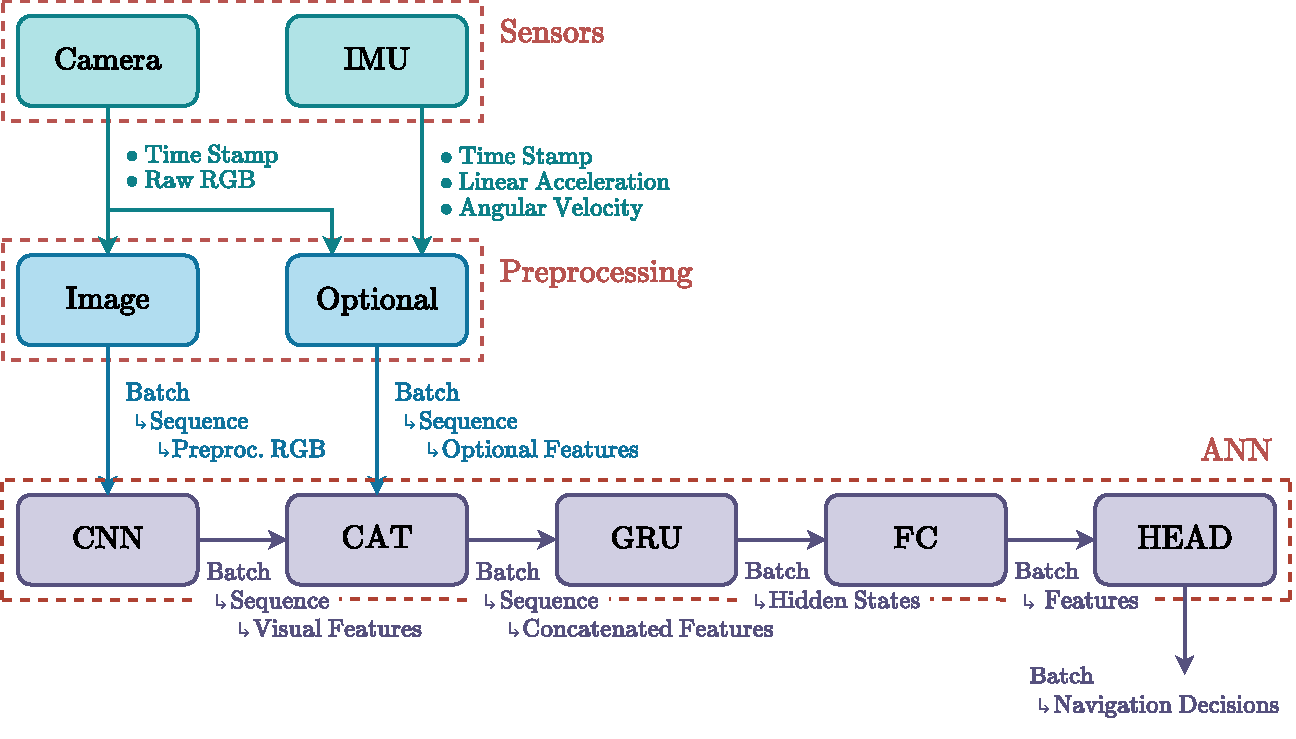
\includegraphics[width=1.0\textwidth]{own/ann_module.drawio.pdf}
    \caption[
        Information flow of the navigation decision-making
    ]{
        Information flow of the navigation decision-making
    \label{fig:perception_and_reasoning}
    }
\end{figure}


The ANN module learns by
imitation with dataset aggregation
(see section \ref{sec:imitation_learning} for background).
Thereby, the dataset is aggregated from samples demonstrated by the expert
system (see section \ref{sec:expert_system}).
Each sample is a pair of an input sequence and a single label.
For the individual ANN variant,
the user specifies the sequence length of the samples
\begin{equation} \label{eq:seq_len}
    \seqLen \in \setOfAllPosInts.
\end{equation}
The ANN module is trained on
batches of the aggregated dataset with supervised learning.
The user specifies the batch size
\begin{equation}
    \batchSize \in \setOfAllPosInts.
\end{equation}
The submodules prior to the GRU submodule (CNN and CAT)
have no sequential awareness and, thus, 
process sequence elements in parallel like batch elements.
In contrast, the GRU submodule
operates in many-to-one mode,
whereby each input sequence of feature vectors is mapped to a 
single non-sequential output feature vector.
The subsequent submodules (FC and HEAD)
then process batches of non-sequential data, 
as is common in conventional feedforward networks.
In this sense,
the GRU submodule is mandatory in case the user specifies
$\seqLen > 1$ for the samples of the training dataset.

At racing,
when the autonomous navigation method flies the drone through the racetrack,
the ANN module makes navigation decisions 
in real-time at the user-specified frequency
$\mainFreq$ with the batch size and sequence length 
of the input
$\batchSize = \seqLen =1$.
The GRU submodule (if activated in the specific variant) 
hence operates in one-to-one mode,
i.e., 
each single non-sequential input feature vector
is mapped to a single non-sequential output feature vector.
Since the single input feature vectors 
trace back to the sensor data coming in at a fixed frequency,
they, as a whole, constitute a time series,
on which the GRU submodule can build up memory
% in its hidden state
as learned during the training on the sequences of the specified length.
As a result, both, the current and past sensor data, 
influence the current navigation decision.





%%%%%%%%%%%%%%%%%%%%%%%%%%%%%%%%%%%%%%%
\paragraph*{Input Preprocessing} ${}$\\
The drone's onboard camera 
outputs raw RGB images
\begin{equation}
    \rawRGB \in \setOfInts{0, \dots, \rawRGBFullInt}^{
        3 \times \rawRGBHeight \times \rawRGBWidth}
\end{equation}
where 
$\rawRGBFullInt$ (usually $= 255$) is the full pixel intensity 
and
$\rawRGBHeight \times \rawRGBWidth$
is the image size.
The latest raw RGB image is preprocessed in two steps
before being fed to the CNN submodule.
First, the pixel intensities are normalized by the full intensity 
$\rawRGBFullInt$ with the aim
to accelerate the convergence of the loss during training.
Second, the image is sized down 
preserving its aspect ratio
with the user-specified factor $\resizeFact$.
Besides significantly accelerating the training,
this step makes training on longer sequences possible
in the first place by reducing GPU memory usage.
The resulting preprocessed RGB image is
\begin{equation} \label{eq:rgb_preproc}
    \preprocRGB{} \in \setOfInts{\frac{i}{\rawRGBFullInt}}_{
        i \in \setOfInts{0, \dots, \rawRGBFullInt}
    }^{
        3 \times 
        \floor{\resizeFact \cdot \rawRGBHeight} \times 
        \floor{\resizeFact \cdot \rawRGBWidth}
    }
\end{equation} 
where $\floor{\placeholder}$ denotes the operation of rounding down to the nearest integer.



The available optional input features are
\begin{itemize}
    \item the time step
    $\rawRGBTimeStep$
    between the stamps of the raw RGB images processed
    at the previous and the current inference
    \item the latest estimate from the drone's onboard IMU
    (inertial measurement unit) 
    comprising the drone's linear acceleration
    $\IMULinAcc \in \R{3}$
    and angular velocity
    $\IMUAngVel \in \R{3}$
    in the local reference system
    \item the time step
    $\IMUTimeStep$
    between the stamps of the IMU estimates
    processed at the previous and the current inference.
\end{itemize}
The user-activated optional inputs are stacked into the optional input vector
before being fed to the CAT submodule.
For example, the fully activated optional input vector is
\begin{align} \label{eq:opt_inp_vec}
    \optFeatVec{} =
    \begin{bmatrix}
        \rawRGBTimeStep \\
        \IMULinAcc \\
        \IMUAngVel \\
        \IMUTimeStep
    \end{bmatrix}.
\end{align}








%%%%%%%%%%%%%%%%%%%%%%%
\paragraph*{CNN Submodule} ${}$\\
The CNN (convolutional neural network) submodule 
extracts visual features of images.
This submodule is implemented with the backbone
of any user-selected TorchVision
classification model\footnote{
    \url{https://pytorch.org/vision/stable/models.html}, visited on 23/08/2022
},
which is obtained by removing the last layer of the model.
In addition, the user specifies whether the backbone
initializes with pretrained weights and whether
the weights of the backbone are trainable.
Since CNN backbones are only applied in this thesis, 
their corresponding mapping is 
regarded as a black box 
\begin{align} \label{eq:CNN}
    \CNNMap 
    :
    \R{\CNNNumC \times \CNNHeight \times \CNNWidth} 
    \rightarrow 
    \R{\CNNOutp}
    ;\quad 
    \img[]{}{}{}{}
    \mapsto 
    \visFeatVec{}
    .
\end{align}
The backbone implementation adapts to the inputted image
in terms of 
the number of channels $\CNNNumC$,
height $\CNNHeight$
and width $\CNNWidth$.
The backbone's output dimensionality 
$\CNNOutp$
is fixed by the design of its last layer.
The user specifies

The CNN submodule inputs
a batch of sequences of preprocessed RGB images 
(equ. \ref{eq:rgb_preproc}) 
\begin{equation}
    \series{\preprocRGB{t}}_{t \in \setOfInts{1, \dots, \seqLen}, i}
    ,\quad 
    i \in \setOfInts{1, \dots, \batchSize}.
\end{equation}
As it processes the individual sequence elements 
unrelated in parallel like batch elements,
the CNN submodule maps each image of the input batch 
to an individual visual feature vector in the output batch
\begin{equation} \label{eq:cnn_output}
    \series{\visFeatVec{t}}_{t \in \setOfInts{1, \dots, \seqLen}, i}
    ,\quad 
    i \in \setOfInts{1, \dots, \batchSize}.
\end{equation}
The number of trainable parameters $\CNNNumP$ of the CNN submodule 
depends on the user-selected TorchVision model.




%%%%%%%%%%%%%%%%%%%%%%%
\paragraph*{CAT Submodule} ${}$\\
The CAT submodule concatenates
two feature vectors
\begin{align} \label{eq:cat}
    \CATMap
    :
    \tuple{\R{\CATInp{1}}, \R{\CATInp{2}}}
    \rightarrow 
    \R{\CATInp{1} + \CATInp{2}}
    ;\quad
    \tuple{\featvec[]{}{1}{}{}, \featvec[]{}{2}{}{}}
    \mapsto
    \begin{bmatrix}
        \featvec[]{}{1}{}{} \\ \featvec[]{}{2}{}{}
    \end{bmatrix}
\end{align}
where the input dimensionalities
$\mathbb{R}^{\num[]{\cat}{1}{}{}}$
and
$\mathbb{R}^{\num[]{\cat}{2}{}{}}$
adapt to the number of features of the input.
This submodule applies to each
visual feature vector 
outputted by the CNN submodule 
(see equ. \ref{eq:cnn_output})
and optional input feature vector
\begin{equation} \label{eq:batch_opt}
    \series{\optFeatVec{t}}_{t \in \setOfInts{1, \dots, \seqLen}, i}
    ,\quad 
    i \in \setOfInts{1, \dots, \batchSize}.
\end{equation}
that correspond to the same position in batch and sequence.
Hence, the CAT submodule outputs a batch of sequences
of concatenated feature vectors
\begin{equation} \label{eq:cat_output}
    \series{
        \begin{bmatrix} 
            \visFeatVec{t} \\ \optFeatVec{t}
        \end{bmatrix}
    }_{t \in \setOfInts{1, \dots, \seqLen}, i}
    ,\quad 
    i \in \setOfInts{1, \dots, \batchSize}.
\end{equation}
If the user deactivates all optional inputs,
the CAT submodule also deactivates and recedes to 
the identity map of the CNN submodule output.
Either way, the CAT submodule has zero trainable parameters
\begin{equation}
    \CATNumP = 0.
\end{equation}




\newcommand{\GRULayerMap}[1]{\Func[]{\gru}{#1}{}{}}
\newcommand{\GRUNumLayer}{\num[\user]{\gru}{\layer}{}{}}
\newcommand{\GRUInp}[1]{\num[]{\gru}{\inp,#1}{}{}}
\newcommand{\GRUHiddenSize}{\num[\user]{\gru}{\hidden}{}{}}

\newcommand{\GRUMap}{\Func[]{\gru}{}{}{}}
\newcommand{\GRUDropout}{\underline\delta}
\newcommand{\GRUDropoutP}{\prob[\user]{\gru}{}{}{}}
\newcommand{\GRUNumP}{\num[]{\gru}{\params}{}{}}

%%%%%%%%%%%%%%%%%%%%%%%
\paragraph*{GRU Submodule} ${}$\\
The GRU (gated recurrent unit) submodule
is implemented using the PyTorch
multi-layer GRU\footnote{
    \url{https://pytorch.org/docs/stable/generated/torch.nn.GRU.html}, visited on 24/08/2022
},
which integrates the GRU \cite{Cho2014} 
introduced in section \ref{sec:gru} on each layer.
As a quick reminder, 
the single layer GRU 
has the ability to comprehend temporal relations within sequences.
Each layer 
$l \in \setOfInts{1, \dots, \GRUNumLayer}$ 
processes an input sequence by
iterating through it
$t \in \setOfInts{1, \dots, \seqLen}$ 
mapping the current sequence element
and the layer's previous hidden state
to the current hidden state (see equ. \ref{eq:gru_layer_current_hidden})
\begin{align}
    \GRULayerMap{l}
    :
    \tuple{
        \R{\GRUInp{l}}, 
        \setR{-1, 1}^{\GRUHiddenSize}
    }
    \rightarrow 
    \setR{-1, 1}^{\GRUHiddenSize}
    ;\quad
    \tuple{\featvec[]{(l)}{t}{}{}, \hiddenstate[]{(l)}{t-1}{}{}}
    \mapsto
    \hiddenstate[]{(l)}{t}{}{}.
\end{align}
Thereby, $\hiddenstate[]{(l)}{0}{}{}$ is either initialized with zeros 
or corresponds to the last computed hidden state from the last inference.
 In the multi-layer GRU,
each layer maintains its own hidden state.
The user specifies the number of layers 
$\GRUNumLayer$
and the hidden size 
$\GRUHiddenSize$ (i.e., dimensionality) shared by all hidden states.
While the first GRU layer inputs the elements of the given input sequence,
all subsequent layers input the hidden state from the previous layer subject to dropout
\begin{align} \label{eq:gru}
    \GRUMap
    :\ &
    \tuple{
        \R{\GRUInp{1}},
        \setR{-1, 1}^{\GRUHiddenSize \times \GRUNumLayer}
    }
    \rightarrow 
    \setR{-1, 1}^{\GRUHiddenSize}
    \nonumber \\
    &\tuple{
        \featvec[]{}{t}{}{}, 
        \hiddenstate[]{(1)}{t-1}{}{},
        \dots,
        \hiddenstate[]{(\GRUNumLayer)}{t-1}{}{}
    }
    \mapsto 
    \hiddenstate[]{(\GRUNumLayer)}{t}{}{} =
    \dots
    \nonumber \\
    \dots &\GRULayerMap{\GRUNumLayer} \tuple{
        \GRUDropout \odot
        \GRULayerMap{\GRUNumLayer - 1} \tuple{
            \GRUDropout \odot
                \dots \GRULayerMap{1} \tuple{
                    \featvec[]{}{t}{}{}
                    ,
                    \hiddenstate[]{(1)}{t-1}{}{}
                }
            ,
            \hiddenstate[]{(\GRUNumLayer-1)}{t-1}{}{}
        },
        \hiddenstate[]{(\GRUNumLayer)}{t-1}{}{}
    }
    .
\end{align}
Dropout is a measure that prevents ANNs from overfitting 
to their provided training data.
At training, 
it randomly sets entries of a feature vector to zero 
while maintaining the vector's signal strength on average
in order to force the ANN to learn the extraction of stand-alone features 
whose informative value is independent of the other extracted features \cite{Hinton2012}.
Mathematically, dropout applied on a hidden state (or feature vector)
is calculated with the Hadamard product (denoted with $\odot$)
of that hidden state and the vector $\GRUDropout$ of same dimensionality 
whose entries, for every calculation, 
are random variables resampled 
from a Bernoulli distribution
with a user-specified probability
\begin{equation}
    P \left( \delta_i = 0 \right) = \GRUDropoutP
    ,\quad
    P \left( \delta_i = \frac{1}{1-\GRUDropoutP} \right) = 1 - \GRUDropoutP
    .
\end{equation}
At racing, the dropout probability is null
whereby the dropout is deactivated.

As the $l$-th GRU layer has $3\GRUHiddenSize (\GRUInp{l} + \GRUHiddenSize + 2)$
trainable parameters (see equ. \ref{eq:gru_layer_nparams}),
the total number of trainable parameters of the GRU submodule is
\begin{align} \label{eq:gru_param}
    \GRUNumP = 3\GRUHiddenSize \tuple{
        (\GRUInp{1} + \GRUHiddenSize + 2)
        + 
        (\GRUNumLayer -1)
        (2\GRUHiddenSize + 2)
    }.
\end{align}

The GRU submodule operates in many-to-one mode at training or 
one-to-one mode at racing where the length of the input sequences is one.
Either way, the GRU submodule maps its input batch
(see equ. \ref{eq:cat_output})
to a batch of last hidden states of the last layer
\begin{equation}
    \hiddenstate[]{(\GRUNumLayer)}{\seqLen, i}{}{}
    , \quad i \in \setOfInts{1, \dots, \batchSize}
    .
\end{equation}




\newcommand{\normDesSpeed}{\speed[\norm]{\drone}{\desired}{}{}}
\newcommand{\waypIRS}{\pos[]{\wayp}{}{\irs}{}}
\newcommand{\headNavDec}{(\normDesSpeed, \waypIRS)}

\newcommand{\desAngVel}{\angvel[]{\drone}{\desired}{\lrs}{}}
\newcommand{\desAngAcc}{\angvel[\dot]{\drone}{\desired}{\lrs}{}}
\newcommand{\desColThrust}{\anything[]{\drone}{\desired}{}{}{c}}
\newcommand{\headCtrlCmd}{(\desAngVel, \desAngAcc, \desColThrust)}

\newcommand{\headMap}{\Func[]{\head}{}{}{}}
\newcommand{\headIn}{\num[]{\head}{\inp}{}{}}
\newcommand{\headOut}{\num[]{\head}{\outp}{}{}}
\newcommand{\headMat}{\underline{\underline A}^\head}
\newcommand{\headBias}{\underline{b}^\head}
\newcommand{\headAct}{\func[\user]{\head}{}{}{}}
\newcommand{\headParam}{\num[]{\head}{\params}{}{}}


\newcommand{\fcLayer}{\num[\user]{\fc}{\layer}{}{}}
\newcommand{\fcIn}[1]{\num[]{\fc}{\inp, #1}{}{}}
\newcommand{\fcOut}{\num[\user]{\fc}{\widthh}{}{}}
\newcommand{\fcMap}[1]{\Func[]{\fc}{#1}{}{}}
\newcommand{\fcMat}[1]{\underline{\underline A}^\fc_{#1}}
\newcommand{\fcBias}[1]{\underline{b}^\fc_{#1}}
\newcommand{\fcDropout}{\underline{\delta}^\fc}
\newcommand{\fcAct}{\func[\user]{\fc}{}{}{}}
\newcommand{\fcDropoutProb}{\prob[\user]{\fc}{}{}{}}
\newcommand{\fcParam}{\num[]{\fc}{\params}{}{}}

\paragraph*{FC Submodule}$\ $\\
The FC submodule performs the function
of increasing the general complexity of the ANN module.
It consists of multiple fully connected layers.
Each layer 
$ l \in \setOfInts{1, \dots, \fcLayer}$ 
applies
an activation, 
dropout
and a biased linear transformation
on the input feature vector
\begin{align} \label{eq:fc_layer}
    \fcMap{l}
    :\ &
    \R{\fcIn{l}} \rightarrow \R{\fcOut}
    ;\quad 
    \featvec[]{}{}{}{} \mapsto
    \fcMat{l} \cdot \fcDropout \odot
    \hadfct{\fcAct} \left(\featvec[]{}{}{}{}\right)
    + \fcBias{l}
    .
\end{align}
In the multi-layer FC submodule, the first layer inputs 
the given input feature vector,
whereas all subsequent layers input the output from the previous layer
\begin{align} \label{eq:fc}
    \fcMap{}
    :\
    \R{\fcIn{1}} \rightarrow \R{\fcOut}
    ;\quad 
    \featvec[]{}{}{}{} \mapsto
    \fcMap{\fcLayer} \tuple{
        \fcMap{\fcLayer - 1} \tuple{
            \dots \fcMap{1} \tuple{
                \featvec[]{}{}{}{}
            }
        }    
    }
    .
\end{align}
For the FC submodule,
the user specifies:
\begin{itemize}
    \item the number of layers $\fcLayer$
    \item the width $\fcOut$, i.e., output dimensionality shared by all layers
    \item the activation function $\fcAct : \R{} \rightarrow \R{}$
    from the non-linear activations implemented in PyTorch\footnote{
        \url{https://pytorch.org/docs/stable/nn.html}, visited on 03/07/2022
    },
    which applies element-wise on the input feature vector (denoted with the overset ${}^\odot$)
    \item the dropout probability $\fcDropoutProb \in \setR{0,1}$,
    i.e., the probability to resample an entry of the vector 
    $\fcDropout$ with zero
    
    
\end{itemize}
The input dimensionality of a layer
adapts to the number of features in the given input vector.
For the first layer, it adapts to the feature vector
forwarded to the FC submodule
$\fcIn{1} = \dim \left(\featvec[]{}{}{}{}\right)$.
For all subsequent layers $l \ge 2$,
it adapts to the width of the FC submodule $ \fcIn{l} = \fcOut$.
The biased linear transformation of the $l$-th layer
consists of the multiplication with the matrix of trainable weights
and the addition of the vector of trainable biases
\begin{equation}
    \fcMat{l} \in \R{\fcIn{l} \times \fcOut}
    , \quad
    \fcBias{l} \in \R{\fcOut}
    .
\end{equation}
As a single layer therewith has $\tuple{\fcIn{l} + 1} \fcOut$
trainable parameters,
the total number of trainable parameters of the FC submodule is
\begin{align} \label{eq:fc_param}
    \fcParam = \tuple{
        \fcIn{1} + 1 + 
        \tuple{\fcLayer -1} \tuple{\fcOut +1}
    } \fcOut
    .
\end{align}
The FC submodule maps
the batch of hidden states
outputted by the GRU submodule
to the batch of feature vectors
\begin{equation}
    \fcMap{} \tuple{\hiddenstate[]{}{}{}{}}_i
    , \quad
    i \in \setOfInts{1, \dots, \batchSize}
    .
\end{equation}






\paragraph*{HEAD Submodule}$\ $\\
The mandatory HEAD submodule
performs the function of mapping
to the final output of the ANN module.
Depending on the user's selection,
the final output is either a navigation decision or a control command.
A navigation decision 
\begin{equation} \label{eq:head_nav_dec}
    \headNavDec
\end{equation}
comprises a normalized desired speed 
$\normDesSpeed \in \setR{0,1}$
of the drone
and a waypoint
$\waypIRS \in \setR{\text{-}1,1}$
in the image reference system
(see fig. \ref{fig:image_reference_system}).
A control command 
\begin{equation} \label{eq:head_ctrl_cmd}
    \headCtrlCmd
\end{equation}
comprises the desired angular velocity
$\desAngVel$
and acceleration
$\desAngAcc$
of the drone in the local reference system 
(see fig. \ref{fig:local_reference_system})
as well as the desired collective thrust 
$\desColThrust$
of the drone's rotors.
In the limited scope of this master's thesis,
the control command output option,
which is a shortcut to the position controller output 
(see section \ref{sec:control_stack}),
is only partly implemented and 
not examined in the experiments in section \ref{maintwo}.

The head submodule
corresponds to a single layer of the FC submodule
without dropout (see equ. \ref{eq:fc_layer})
as it
applies an activation and a biased linear transformation on the
input feature vector
\begin{align} \label{eq:head}
    \headMap
    :\ 
    \R{\headIn}
    \rightarrow 
    \R{\headOut}
    ;\quad 
    \featvec[]{}{}{}{}
    \mapsto
    \headMat \cdot \hadfct{\headAct}\left(\featvec[]{}{}{}{}\right)
    + \headBias
    .
\end{align}
For the HEAD submodule, the user selects
the activation function $\fcAct : \R{} \rightarrow \R{}$
from the non-linear activations implemented in PyTorch\footnote{
        \url{https://pytorch.org/docs/stable/nn.html}, visited on 03/07/2022
    },
which applies element-wise on the input feature vector (denoted with the overset ${}^\odot$).
The input dimensionality adapts to the
number of features of the given input vector
\begin{equation}
    \headIn
    =
    \dim \left(\featvec[]{}{}{}{}\right),
\end{equation}
whereas the output dimensionality
adapts to the user-selected output option
\begin{equation}
    \headOut
    = 
    \begin{cases}
        3
        ,\quad 
        \text{if navigation decision} 
        \\
        7
        ,\quad 
        \text{if control command.} 
    \end{cases}
\end{equation}
The total number of trainable parameters of the HEAD submodule is
\begin{equation} \label{eq:head_param}
    \headParam = \left( \headIn + 1 \right) \headOut
    .
\end{equation}






%CNN: torch vision model, pretrained, trainable, adapt to any RGB size
%CAT: CNN output , CAT input , one vector
%GRU: hidden size, num_layers, bias, dropout
%FC: width, num_layers, act fct, bias
%HEAD: output size, act fct, bias
%GRAPH
%
%loss optimizer learnrate











\section{Planning Module}
The planning module performs the task of path planning
within the autonomous navigation method.
At the user-specified main frequency 
$\freq[\user]{\main}{}{}{}$,
the planning module 
samples states from its local trajectory
and forwards them as reference to the control module.
Every $\num[\user]{\text{plan}}{}{}{}$-th (user-specified) iteration,
the planning module re-computes its local trajectory
on the basis of its input,
i.e., the latest navigation decision and the latest drone state estimate. 
%These trajectories, generated by the planning module, 
%are referred to as local trajectories
%to distinguish them from the expert system's global trajectory
%used when generating training data for the ANN module (see XX).

The latest navigation decision
stems from either the ANN module
or, if it has intervened at training data generation,
the expert system.
A navigation decision comprises the normalized desired speed 
and the waypoint in the image reference system
\begin{equation}
    (
        \speed[\norm]{\drone}{\desired}{}{}
        ,\ 
        \pos[]{\wayp}{}{\irs}{}
    ).
\end{equation}
The latest drone state estimate stems from the state estimation system.
In simulation, the estimate may correspond to the ground-truth state.
A drone state estimate includes position, velocity and acceleration
with respect to the global reference system
\begin{equation} \label{eq:drone_state}
    \pos[]{\drone}{}{\grs}{}
    ,\ 
    \vel[]{\drone}{}{\grs}{}
    ,\ 
    \acc[]{\drone}{}{\grs}{}.
\end{equation}


At a fraction of the main frequency, i.e.,
$\freq[\user]{\main}{}{}{} / \num[\user]{\text{plan}}{}{}{}$, 
the planning module takes the following 5 steps 
to re-compute its local trajectory.
\begin{enumerate}
    \item Compute the desired speed
    \begin{equation} \label{eq:planning_des_speed}
        \speed[]{\drone}{\desired}{}{}
        = 
        \maxof{
            \speed[\user]{\drone}{\mnm}{}{}
        }{
            \speed[\user]{\drone}{\mxm}{}{}
            \cdot 
            \speed[\norm]{\drone}{\desired}{}{}
        }.
    \end{equation}
    The normalized, desired speed 
    $\speed[\norm]{\drone}{\desired}{}{} \in \left[0, 1\right]$ 
    of the navigation decision
    is rescaled by its upper bound, 
    the user-specified drone's maximum speed 
    $\speed[\user]{\drone}{\mxm}{}{}$.    
    The user-specified drone's minimum speed 
    $\speed[\user]{\drone}{\mnm}{}{}$
    lower-bounds the desired speed.

    \item Compute the drone's distance to the waypoint 
    \begin{equation}
        \dist[]{\dronetowayp}{}{}{}
        = 
        \maxof{
            \dist[\user]{\dronetowayp}{\mnm}{}{}
        }{
            \minof{
                \speed[]{\drone}{\desired}{}{}
                \cdot
                \dur[\user]{\dronetowayp}{}{}{}
            }{
                \dist[\user]{\dronetowayp}{\mxm}{}{}
            }
        }.
    \end{equation}
    The desired speed 
    $\speed[]{\drone}{\desired}{}{}$ 
    is integrated over the user-specified duration
    $\dur[\user]{\dronetowayp}{}{}{}$.
    The result is bounded to the interval spanned 
    by the user-specified minimum
    $\dist[\user]{\dronetowayp}{\mnm}{}{}$
    and maximum
    $\dist[\user]{\dronetowayp}{\mxm}{}{}$
    distance.

    \item Compute the waypoint with respect to the global reference system
    \begin{equation} \label{eq:pl_global_wayp}
        \pos[]{\wayp}{}{\grs}{}
        = 
        \trafo[]{}{\grs\irs}{}{} \left(
            \dist[]{\dronetowayp}{}{}{}
            ,\ 
            \pos[]{\wayp}{}{\irs}{}
        \right).
    \end{equation}
    The transformation
    $\trafo[]{}{\grs\irs}{}{}$
    (see equ. \ref{eq:global_image_transformations})
    back-projects the waypoint
    $\pos[]{\wayp}{}{\irs}{}$ 
    of the navigation decision
    from the 2D image to the 3D global reference system.
    Thereby, the drone's distance 
    $\dist[]{\dronetowayp}{}{}{}$
    to the waypoint
    constitutes the back-projection length.
    
    \item Set the starting time of the local trajectory to the current time
    \begin{equation}
        \timepnt[]{\loctraj}{0}{}{} = t
    \end{equation}
    and compute the duration of the local trajectory 
    \begin{equation}
        \dur[]{\loctraj}{}{}{}
        = 
        \frac{
            \dist[]{\dronetowayp}{}{}{}
        }{
            \minof{
            \speed[]{\drone}{\desired}{}{}
            }{
                %\speed[]{\drone}{}{}{} 
                \left\|
                    \vel[]{\drone}{}{\grs}{}
                \right\|_2
                + 
                \speed[\user]{\drone}{\Delta}{}{}
            }
        }.
    \end{equation}
    The drone's distance 
    $\dist[]{\dronetowayp}{}{}{}$
    to the waypoint is divided 
    by the slowest of either the desired speed
    $\speed[]{\drone}{\desired}{}{}$
    or the latest drone speed estimate
    $\left\|\vel[]{\drone}{}{\grs}{}\right\|_2$
    plus a user-specified speed increment
    $\speed[\user]{\drone}{\Delta}{}{}$.
    By relating the desired to the estimated speed,
    excessive speed increases
    potentially violating the drone's dynamic limitations
    can be prevented.

    \item Compute the local trajectory 
    \begin{align} \label{eq:loc_traj}
        \pos[]{\loctraj}{}{\grs}{}
        :\ 
        &\left[0, \dur[]{\loctraj}{}{}{}\right] \rightarrow \mathbb{R}^3
        ;\quad
        %\nonumber \\
        \timepnt[]{}{}{}{}
        \mapsto
        \pos[]{\loctraj}{}{\grs}{}(\timepnt[]{}{}{}{})
    \end{align}
    starting in the latest drone state estimate
    $\pos[]{\drone}{}{\grs}{}
    ,\ 
    \vel[]{\drone}{}{\grs}{}
    ,\ 
    \acc[]{\drone}{}{\grs}{}$
    and ending in the global waypoint
    $\pos[]{\wayp}{}{\grs}{}$
    with unconstrained velocity and acceleration.
    The implementation\footnote{
            \url{https://github.com/markwmuller/RapidQuadrocopterTrajectories}, visited on 17/08/2022
    } 
    of the algorithm of Mueller et. al. \cite{Mueller2013}
    is deployed to find the polynomial trajectory with minimum jerk
    (third time derivative of position)
    by solving the optimization problem
    \begin{align} \label{eq:loc_traj_opt_prob}
        &\qquad \min 
        \int_0^{\dur[]{\loctraj}{}{}{}}
            \left\|
                \pos[\dddot]{\loctraj}{}{\grs}{}(\timepnt[]{}{}{}{})
            \right\|^2_2
        \text d \timepnt[]{}{}{}{}
        \nonumber \\
        \text{s.t.}\quad
        & \pos[]{\loctraj}{}{\grs}{}(0) = \pos[]{\drone}{}{\grs}{}
        \qquad\qquad \pos[]{\loctraj}{}{\grs}{}(\dur[]{\loctraj}{}{}{}) = \pos[]{\wayp}{}{\grs}{}
        \nonumber \\
        & \pos[\dot]{\loctraj}{}{\grs}{}(0) = \vel[]{\drone}{}{\grs}{}
        \qquad\qquad \pos[\dot]{\loctraj}{}{\grs}{}(\dur[]{\loctraj}{}{}{}) \text{ free}
        \nonumber \\
        & \pos[\ddot]{\loctraj}{}{\grs}{}(0) = \acc[]{\drone}{}{\grs}{}
        \qquad\qquad \pos[\ddot]{\loctraj}{}{\grs}{}(\dur[]{\loctraj}{}{}{}) \text{ free}.
    \end{align}
    The drone's dynamic limitations
    are only taken into account in subsequent feasibility checks 
    and are exempt from the above optimization problem.
    This allows the algorithm to solve the optimization problem in closed form
    which is characterized by low computational effort.
    The algorithm therewith qualifies 
    to run at the relatively high frequencies
    required by the autonomous navigation method.
\end{enumerate}


At the main frequency $\freq[\user]{\main}{}{}{}$, 
the planning module takes the following 2 steps to sample 
a reference state from its local trajectory.
\begin{enumerate}
    \item Compute the time point of the reference state
    \begin{equation}
        \timepnt[]{\loctraj}{}{}{} 
        = 
        t - \timepnt[]{\loctraj}{0}{}{} + 1/\freq[\user]{\main}{}{}{}.
    \end{equation}
    The actual time $t$ is related to the starting time 
    $\timepnt[]{\loctraj}{0}{}{}$
    of the local trajectory,
    whose time domain starts at zero.
    The addition of the main period
    $1/\freq[\user]{\main}{}{}{}$
    ensures that the sampled reference state remains prospective at all times.
    \item Sample the current reference state from the local trajectory
    \begin{align} \label{eq:ref_state}
        \pos[]{\text{ref}}{}{\grs}{} 
        &= 
        \pos[]{\loctraj}{}{\grs}{}(\timepnt[]{\loctraj}{}{}{})
        \nonumber \\
        \vel[]{\text{ref}}{}{\grs}{} 
        &= 
        \pos[\dot]{\loctraj}{}{\grs}{}(\timepnt[]{\loctraj}{}{}{})
        \nonumber \\
        \acc[]{\text{ref}}{}{\grs}{} 
        &= 
        \pos[\ddot]{\loctraj}{}{\grs}{}(\timepnt[]{\loctraj}{}{}{})
        \nonumber \\
        \jerk[]{\text{ref}}{}{\grs}{} 
        &= 
        \pos[\dddot]{\loctraj}{}{\grs}{}(\timepnt[]{\loctraj}{}{}{})
        \nonumber \\
        \ang[]{\text{ref}}{z}{}{}
        &=
        \mathrm{atan2}\left(
            \speed[]{\text{ref}}{y}{\grs}{}
            ,
            \speed[]{\text{ref}}{x}{\grs}{}
        \right).
    \end{align}
    The reference yaw $\ang[]{\text{ref}}{z}{}{}$ is set so that
    the drone and therewith its onboard camera 
    point in the direction of flight movement.
\end{enumerate}











\section{Control Stack} \label{sec:control_stack}
Within the autonomous navigation method, 
the control stack takes on the task of 
flying the drone as planned.
To do this, the control stack
generates the inputs for the motors attached to the drone's rotors,
which consequently track the latest reference state
(equ. \ref{eq:ref_state})
from the planning module.
In the simulations of this thesis,
the control stack is realized with the RPG Quadrotor Control \footnote{
        \url{https://github.com/uzh-rpg/rpg_quadrotor_control}, visited on 17/08/2022
} implementation
(see fig. \ref{fig:control_module}).
Since this thesis centers on the reasoning aspect of autonomous navigation, 
only an overview of the deployed control stack is presented here.
The reader may consult the provided references for more details
on the control.

\begin{figure}
    \centering
    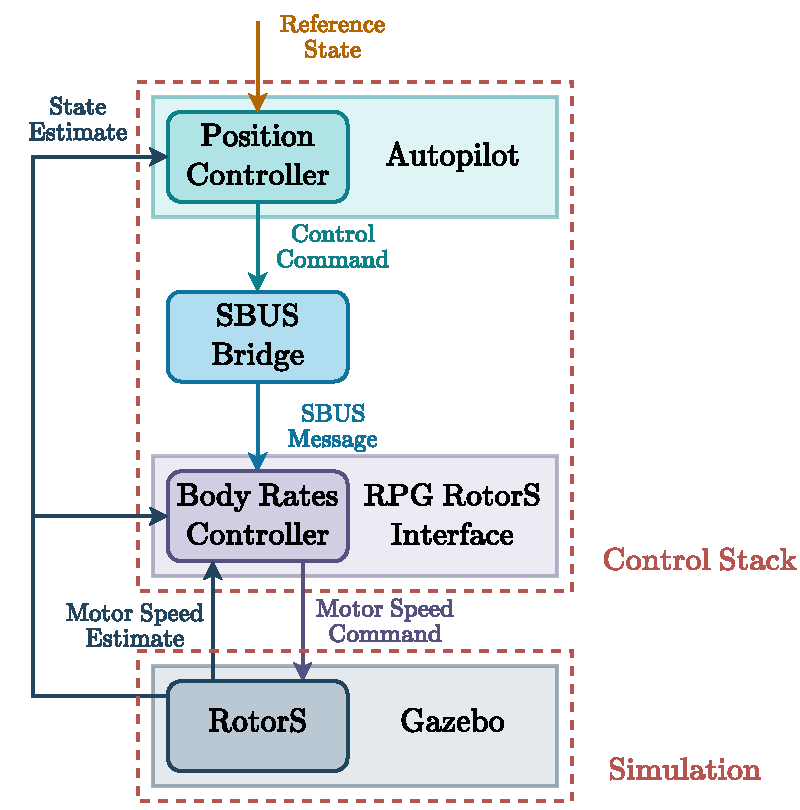
\includegraphics[width=0.7\textwidth]{own/control_module.drawio.pdf}
    \caption[
        The control stack in simulation.
    ]{
        The control stack in simulation.
        \label{fig:control_module}}
\end{figure}

The RPG Quadrotor Control implementation,
which includes the autopilot, the SBUS bridge and and the RPG RotorS interface,
basically executes two feedback control loops in a cascade.
The autopilot integrates the position controller 
that runs the control algorithm of Faessler at al. proposed in \cite{Faessler2018}.
Based on the latest reference state and the fed back drone state estimates,
the position controller generates high-level control commands.
A control command comprises 
the collective thrust of the drone's rotors 
as well as the drone's angular velocity and acceleration.
The SBUS bridge converts each incoming control command
into an SBUS message and forwards this message to the
RPG RotorS interface.
The RPG RotorS interface integrates the body-rate controller
that runs the control algorithm of Faessler at al. proposed in \cite{Faessler2017}.
Based on the latest high-level control command 
as well as the fed back drone state and motor speed estimates,
the body-rate controller generates low-level motor speed commands.
These commands are forwarded to RotorS for execution.
RotorS, developed by Furrer et al. \cite{Furrer2016},
is plugged into the Gazebo \footnote{
    \url{https://gazebosim.org/home}, visited on 18/08/2022
}
simulator to model the drone's physics 
and to provide the controllers with
drone state and motor speed estimates.

In real-world, the drone's flight controller would replace the 
RPG RotorS interface in order to generate hardware-specific low-level
motor commands based on the latest SBUS message from the SBUS bridge.








\section{Expert System} \label{sec:expert_system}
%In contrast to the ANN module,
%the expert system derives its navigation decisions 
%not from onboard sensor data but from its knowledge base.
%The task of the ANN module 
%is to infer navigation decisions,
%i.e., the inputs of the planning module,
%from onboard sensor data.
%In order to make meaningful decisions
%that successfully guide the drone through the racetrack,
%the ANN module must be previously trained on training data 
%of sufficient quantity and quality.
%To guarantee both,
%the training data is automatically generated 
%while the drone is flying through the racetrack.
%At training data generation (see XXX),
%the expert system undertakes the task
%of the completely untrained or yet insufficiently trained ANN module
%to make navigation decisions.

In the context of machine learning, 
an expert system is a program that imitates a human expert
in order to solve a problem. 
It comprises a knowledge base,
which stores known facts and rules, and an
inference engine, which infers new facts 
by applying the rules to the known facts \cite{osti_5675197}.

\paragraph*{Problem} $\ $\\
This thesis implements the expert system 
by Kaufmann et al. \cite{Kaufmann2018}
in order to solve the problem of automated navigation decision-making
during the generation of training data for the ANN module.
The training dataset is extended with new samples 
while the drone runs the autonomous navigation method to fly through a racetrack.
The expert system checks the latest navigation decision 
made by the yet partially trained ANN module.
If it does not meet certain requirements,
the expert system intervenes with its own navigation decision.
This, first, keeps the drone on course and, second,
triggers the generation of a new training sample labeled 
with the expert system's navigation decision.

\paragraph*{Knowledge base} $\ $\\
While the ANN module infers navigation decisions from onboard sensor data,
the expert system makes navigation decisions based on its knowledge
which includes the following known facts (\textbf{F*}) and rules (\textbf{R*}).
\begin{itemize}
    
    \item [\textbf{F1}] 
    The planning module's waypoint
    \begin{equation}
        \pos[]{\text{ann}}{\wayp}{\grs}{}
    \end{equation}
     with respect to the global reference system
    (see equ. \ref{eq:pl_global_wayp}) 
    that was computed based
    on the ANN module's latest navigation decision
    (see equ. \ref{eq:head_nav_dec}).
    

    \item [\textbf{F2}] The drone's latest position and quaternion orientation estimate,
    which are provided by the drone's state estimation system and 
    may correspond to ground truth in the simulation
    \begin{equation}
        \pos[]{\drone}{}{\grs}{}
        ,\quad 
        \quat[]{\drone}{}{\grs}{}.
    \end{equation}
    
    \item [\textbf{F3}] The center points of the gates of the racetrack
    \begin{equation}
        \left( 
            \pos[]{\gate}{\idx[]{}{}{}{}}{\grs}{}
        \right)
        _{\idx[]{}{}{}{} \in \left\{0, ..., \num[]{\gate}{}{}{} - 1 \right\}}
    \end{equation}
    and the initial index to the currently targeted gate to be passed next
    \begin{equation}
        \idx[]{\gate}{\target}{}{} \in \left\{0, ..., \num[]{\gate}{}{}{} - 1 \right\}
        .
    \end{equation}

    \item [\textbf{R1}] Compute the global trajectory of the current racetrack
    \begin{align} \label{eq:glo_traj}
        \pos[]{\glotraj}{}{\grs}{}
        :\ 
        &\left[
            \timepnt[]{\gate}{0}{}{}, 
            \timepnt[]{\gate}{\num[]{\gate}{}{}{}}{}{}
        \right] \rightarrow \mathbb{R}^3
        ;\quad
        \timepnt[]{}{}{}{}
        \mapsto
        \pos[]{\glotraj}{}{\grs}{}(\timepnt[]{}{}{}{})
        .
    \end{align}
    The algorithm of Mellinger and Kumar \cite{Mellinger2011}
    finds the minimum snap (fourth time derivative of position) spline trajectory
    \begin{align}
        \pos[]{\glotraj}{}{\grs}{}(\timepnt[]{}{}{}{})
        = \sum_{i = 0}^{\num[]{\gate}{}{}{} - 1}
        \begin{cases}
            \pos[]{\glotraj}{i}{\grs}{}(\timepnt[]{}{}{}{})
            , 
            &t \in \left[\timepnt[]{\gate}{i}{}{}, \timepnt[]{\gate}{i+1}{}{}\right] \\
            0, & \text{else}
        \end{cases}
    \end{align}
    that, traverses through all gate center points (\textbf{F3}),
    each at its corresponding gate time $\timepnt[]{\gate}{i}{}{}$,
    and reconnects to itself at $t=\timepnt[]{\gate}{\num[]{\gate}{}{}{}}{}{}$ at gate $i=0$.
    The entries of the pieces 
    $\pos[]{\glotraj}{i}{\grs}{}(\timepnt[]{}{}{}{})$
    of the spline are polynomials. 
    The user specifies the polynomial order 
    $\num[\user]{\glotraj}{\text{poly}}{}{}$
    of the pieces and
    the continuity order
    $\num[\user]{\glotraj}{\text{cont}}{}{}$
    of the spline. 
    However, since the goal is to minimize snap,
    it is required that 
    $
    \num[\user]{\glotraj}{\text{poly}}{}{}
    \ge \num[\user]{\glotraj}{\text{cont}}{}{} \ge 4
    $.
    The algorithm performs the following two-step iterative optimization.

    First,
    the optimal polynomial coefficients of the spline pieces
    are found for fixed gate arrival times 
    $\timepnt[]{\gate}{i}{}{}$
    by solving the optimization problem
    \begin{align} \label{eq:glo_traj_opt_prob}
        &\qquad \argmin{\pos[]{\glotraj}{}{\grs}{}}
        \int_{\timepnt[]{\gate}{0}{}{}}^{\timepnt[]{\gate}{\num[]{\gate}{}{}{}}{}{}}
            \left\|
                \pos[\ddddot]{\glotraj}{}{\grs}{}(\timepnt[]{}{}{}{})
            \right\|^2_2
        \text d \timepnt[]{}{}{}{}
        \nonumber 
        \\
        \text{s.t.}\quad
        & \pos[]{\glotraj}{}{\grs}{}\left(\timepnt[]{\gate}{i}{}{}\right) = 
            \pos[]{\gate}{\idx[]{}{}{}{}}{\grs}{},
        &&
            \frac{\text d^j \pos[]{\glotraj}{}{\grs}{}}{\text d \timepnt[]{j}{}{}{}} 
            (\timepnt[]{\gate}{i}{}{}) \text{ defined},
        \nonumber \\
        & \idx[]{}{}{}{} \in \left\{0, ..., \num[]{\gate}{}{}{}\right\},
        && j \in \left\{1, ..., \num[\user]{\glotraj}{\text{cont}}{}{}\right\}.
    \end{align}
    Note that, as the spline is closed, 
    the first and last gate equate 
    $\pos[]{\gate}{\num[]{\gate}{}{}{}}{\grs}{} = \pos[]{\gate}{0}{\grs}{}$.
    Morover, the gate times of the very first iteration are 
    approximated with the distances between the gate center points
    divided by the user-specified maximum speed $\speed[\user]{\glotraj}{\mxm}{}{}$ of the trajectory.
    The above optimization problem
    is temporally and spatially de-dimensionalized 
    to increase numeric stability and 
    reformulated as quadratic program,
    which is solved with the Gurobi\footnote{
        \url{https://www.gurobi.com/}, visited on 20/08/2022
    } optimizer.

    Second, the polynomial coefficients of the spline pieces 
    are fixed
    and the inner gate times
    $\timepnt[]{\gate}{i}{}{}$
    are optimized relatively to each other.
    The corresponding optimization problem
    \begin{align}
        &\qquad \argmin{\timepnt[]{\gate}{i}{}{}}
        \int_{\timepnt[]{\gate}{0}{}{}}^{\timepnt[]{\gate}{\num[]{\gate}{}{}{}}{}{}}
            \left\|
                \pos[\ddddot]{\glotraj}{}{\grs}{}(\timepnt[]{}{}{}{})
            \right\|^2_2
        \text d \timepnt[]{}{}{}{}
        \nonumber \\
        \text{s.t.}\quad
        & \timepnt[]{\gate}{i}{}{} < \timepnt[]{\gate}{i+1}{}{},
        \qquad
        \timepnt[]{\gate}{0}{}{},\ \timepnt[]{\gate}{\num[]{\gate}{}{}{}}{}{} \text{ fixed},
        \qquad
        \idx[]{}{}{}{} \in \left\{0, ..., \num[]{\gate}{}{}{} - 1 \right\}
    \end{align}
    is solved by gradient descent with backtracking line search.

    
    
    The two optimization steps are executed iteratively until the cost
    of the first optimization problem converges. 
    Then, the trajectory is temporally and spatially re-dimensionalized
    and temporally scaled to adhere to 
    the user-specified maximum values in terms of 
    speed
    $\speed[\user]{\glotraj}{\mxm}{}{}$, 
    thrust 
    $\scacc[\user]{\glotraj}{\mxm}{}{}$
    and roll-pitch rate 
    $\scangvel[\user]{\glotraj}{\mxm}{}{}$
    along the trajectory. 
    For later use,
    the expert system samples the positions and speeds
    of the global trajectory
    \begin{equation}
        \left( 
            \pos[]{\glotraj}{\idx[]{}{}{}{}}{\grs}{}
        \right)
        _{\idx[]{}{}{}{} \in \left\{0, ..., \num[]{\glotraj}{}{}{} - 1 \right\}}
        ,\quad
        \left( 
            \speed[]{\glotraj}{\idx[]{}{}{}{}}{\grs}{}
        \right)
        _{\idx[]{}{}{}{} \in \left\{0, ..., \num[]{\glotraj}{}{}{} - 1 \right\}}
    \end{equation}
    with $\speed[]{\glotraj}{\idx[]{}{}{}{}}{\grs}{} = 
    \left\| 
        \pos[\dot]{\glotraj}{\idx[]{}{}{}{}}{\grs}{}
    \right\|_2 $.
    The sampling occurs at the
    user-specified frequency
    $\freq[\user]{\glotraj}{}{}{}$,
    which results in
    $\num[]{\glotraj}{}{}{} = \freq[\user]{\glotraj}{}{}{} \cdot 
    \left(\timepnt[]{\gate}{\num[]{\gate}{}{}{}}{}{}
    - \timepnt[]{\gate}{0}{}{}\right)$
    samples.

    
    \item [\textbf{R2}] If the drone is closer to the currently targeted gate 
    than a user-specified distance
    \begin{equation}
        \left\| 
            \pos[]{\gate}{\idx[]{\gate}{\target}{}{}}{\grs}{} - \pos[]{\drone}{}{\grs}{}
        \right\|_2 
        < 
        \dist[\user]{\dronetogate}{}{}{},
    \end{equation}
    increment the index to the currently targeted gate
    \begin{align}
        \idx[]{\gate}{}{}{} &\leftarrow (\idx[]{\gate}{}{}{} + 1) \bmod \num[]{\gate}{}{}{}.
    \end{align}
    
    \item [\textbf{R3}] If the
    planning module's waypoint (\textbf{F1}) computed based on the
    ANN module's latest navigation decision,
    is more distant from the global trajectory (\textbf{R1}) than
    a user-specified margin scaled by
    the user-specified drone's maximum speed, i.e.,
    \begin{equation}
        \argmin{i \in \{0, ..., \num[]{\glotraj}{}{}{} - 1\}}
            \left\| 
                \pos[]{\text{ann}}{\wayp}{\grs}{}
                - 
                \pos[]{\glotraj}{i}{\grs}{}
            \right\|_2
            >
            \dist[\user]{\wayptoglotraj}{\mxm}{}{} \cdot \frac{\speed[\user]{\drone}{\mxm}{}{} +1}{5},
    \end{equation}
    the expert system is required to intervene with its own navigation decision.

    
    \item [\textbf{R4}] Update the index 
    $\idx[]{\glotraj}{\proj}{}{} \in \{0, ..., \num[]{\glotraj}{}{}{} - 1\}$ 
    to the projection state,
    i.e., the state of the global trajectory
    onto which the drone's latest position estimate is projected,
    with the following iterative method.
    Figure \ref{fig:expert_system_projection} 
    schematically illustrates the method with a 2D example.
    \begin{enumerate}
        \item Compute the index to the previous state of the global trajectory,
        by decrementing the index to the projection state
        \begin{equation}
            \idx[]{\glotraj}{\prev}{}{} 
            = 
            (\idx[]{\glotraj}{\proj}{}{} - 1 + \num[]{\glotraj}{}{}{}) 
            \bmod 
            \num[]{\glotraj}{}{}{}.
        \end{equation}
        \item Starting from the previous state, 
        compute the vector to the projection state
        \begin{equation} \label{eq:vec_prev_state_2_proj_state}
            \anything[]{}{}{\grs}{}{\underline a}
            = 
            \pos[]{\glotraj}{\idx[]{\glotraj}{\proj}{}{}}{\grs}{}
            - 
            \pos[]{\glotraj}{\idx[]{\glotraj}{\prev}{}{}}{\grs}{}
        \end{equation}
        and the vector to the current drone position
        \begin{equation} \label{eq:vec_prev_state_2_drone}
            \anything[]{}{}{\grs}{}{\underline b}
            = 
            \pos[]{\drone}{}{\grs}{}
            - 
            \pos[]{\glotraj}{\idx[]{\glotraj}{\prev}{}{}}{\grs}{}.
        \end{equation}
        \item If the scalar product of the vectors 
        $\anything[]{}{}{\grs}{}{\underline a}$ 
        and 
        $\anything[]{}{}{\grs}{}{\underline b}$, 
        both normalized by the length of $\anything[]{}{}{\grs}{}{\underline a}$,
        is less than 1
        \begin{align} \label{eq:norm_dot_prod_criterion}
            \frac{
                \anything[]{}{}{\grs}{}{\underline a} 
                \cdot 
                \anything[]{}{}{\grs}{}{\underline b}
            }{  
                \anything[]{}{}{\grs}{}{\underline a} 
                \cdot 
                \anything[]{}{}{\grs}{}{\underline a}
            } < 1,
        \end{align}
        go to the next step. 
        Else, increment the index to the projection state
        \begin{equation}
            \idx[]{\glotraj}{\proj}{}{} 
            \leftarrow 
            (\idx[]{\glotraj}{\proj}{}{} + 1) \bmod \num[]{\glotraj}{}{}{}
        \end{equation}
        and go back to step 1.
        \item If the drone is 
        within a user-specified distance to the projection state 
        \begin{equation} \label{eq:dist_drone_proj_criterion}
            \left\| 
                \pos[]{\drone}{}{\grs}{}
                - 
                \pos[]{\glotraj}{\idx[]{\glotraj}{\proj}{}{}}{\grs}{}
            \right\|_2 
            \le 
            \dist[\user]{\dronetoproj}{}{}{},
        \end{equation}
        the index 
        $\idx[]{\glotraj}{\proj}{}{}$ 
        to the projection state is found.
        Else, set the index 
        to the state of the global trajectory
        which has the minimum distance to the current drone position
        \begin{equation} \label{eq:proj_idx_with_min_dist}
            \argmin{\idx[]{\glotraj}{\proj}{}{}}
            \left\| 
                \pos[]{\drone}{}{\grs}{}
                - 
                \pos[]{\glotraj}{\idx[]{\glotraj}{\proj}{}{}}{\grs}{}
            \right\|_2.
        \end{equation}
        Due to this step,
        the expert system does not require to know
        the initial index 
        to the projection state.

    \end{enumerate}
    
    

    \begin{figure}
        \centering
        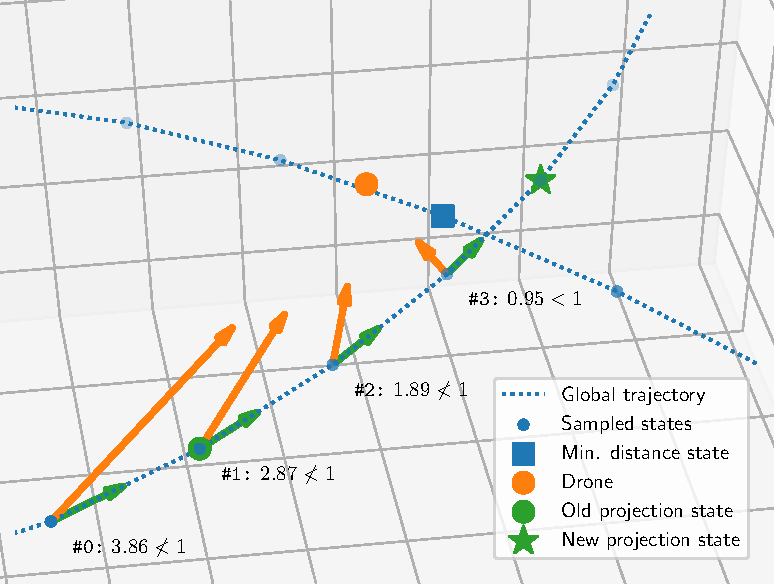
\includegraphics[width=0.9\textwidth]{own/expert_state_projection_3d.pdf}
        \caption[
            Update of the projection state index
        ]{
            Schematic example
            of the update of the projection state index (\textbf{R4}).
            Known are: the positions (blue points) 
            sampled from the global trajectory (blue dotted line),
            the last index to the projection state (green circle)
            and the current position of the drone (orange circle).
            At an iteration,
            the vector from the previous to the projection state 
            (green arrows, equ. \ref{eq:vec_prev_state_2_proj_state})
            and the vector from the previous to the drone position 
            (orange arrows, equ. \ref{eq:vec_prev_state_2_drone})
            are computed.
            Then, the normalized dot product criterion 
            (annotations, equ. \ref{eq:norm_dot_prod_criterion}) 
            is checked. 
            For iteration \#0-2, the criterion is not met.
            Thus, the index to the projection state is incremented
            and another iteration is started.
            At iteration \#3 the criterion is met and the 
            new index to the projection state (green star) is identified
            (assuming the distance criterion 
            (equ. \ref{eq:dist_drone_proj_criterion}) is also met). 
            Note that finding the index to the projection state 
            only with minimum distance 
            (equ. \ref{eq:proj_idx_with_min_dist}) 
            would have failed here,
            since the so indexed state (blue square) 
            belongs to a later or earlier part of the global trajectory 
            which only intersects the current part.
        \label{fig:expert_system_projection}}
    \end{figure}


    
    \item [\textbf{R5}] 
    Update the index 
    $\idx[]{\glotraj}{v}{}{} \in \{0, ..., \num[]{\glotraj}{}{}{} - 1\}$
    to the speed state,
    i.e., the state of the global trajectory
    that is the reference for the normalized speed
    $\speed[\norm]{\expert}{\desired}{}{}$ component
    of the expert system's navigation decision,
    by finding the first state of the global trajectory 
    that follows the projection state
    with a specific distance.
    \begin{enumerate}
        \item Initialize the searched index with the index to the projection state
        \begin{equation}
            \idx[]{\glotraj}{v}{}{} = \idx[]{\glotraj}{\proj}{}{}.
        \end{equation}

        \item Increment the searched index
        \begin{equation}
            \idx[]{\glotraj}{v}{}{} \leftarrow (\idx[]{\glotraj}{v}{}{} + 1) \bmod \num[]{\glotraj}{}{}{}.
        \end{equation}
        \item If the speed state is further 
        from the projection state than a user-specified distance
        \begin{equation}
            \left\| 
                \pos[]{\glotraj}{\idx[]{\glotraj}{v}{}{}}{\grs}{}
                - 
                \pos[]{\glotraj}{\idx[]{\glotraj}{\proj}{}{}}{\grs}{}
            \right\|_2
            > 
            \dist[\user]{\projtospeed}{}{}{}
            .
        \end{equation}
        the searched index is found.
        Else, go back to step 2.
    \end{enumerate}


    \item [\textbf{R6}] 
    Update the index 
    $\idx[]{\glotraj}{\wayp}{}{} \in \{0, ..., \num[]{\glotraj}{}{}{} - 1\}$
    to the waypoint state,
    i.e., the state of the global trajectory
    that is the reference for the image waypoint
    $\pos[]{\expert}{\wayp}{\irs}{}$
    component of the expert system's navigation decision,
    by finding the first state of the global trajectory 
    that follows the projection state
    with a distance to be computed.
    \begin{enumerate}
        \item Set the distance from the projection to the waypoint state
        to the distance from the drone to the closer of
        either the currently or lastly targeted gate.
        However, a user-specified distance constitutes the lower limit
        \begin{align}
            \dist[]{\projtowayp}{}{}{} &= 
            \maxof{
                \dist[\user]{\projtowayp}{\mnm}{}{}
            }{
                \argmin{i} \left\| 
                    \pos[]{\gate}{i}{\grs}{} 
                    - 
                    \pos[]{\drone}{}{\grs}{}
                \right\|_2
            }, 
            \\
            i &\in \left\{ \idx[]{\gate}{\target}{}{}, 
            (\idx[]{\gate}{\target}{}{} - 1 + \num[]{\gate}{}{}{}) 
            \bmod 
            \num[]{\gate}{}{}{}
            \right\}
            .
        \end{align}
        \item Initialize the searched index with the index to the projection state
        \begin{equation}
            \idx[]{\glotraj}{\wayp}{}{} = \idx[]{\glotraj}{\proj}{}{}.
        \end{equation}
        \item Increment the searched index
        \begin{equation}
            \idx[]{\glotraj}{\wayp}{}{} \leftarrow (\idx[]{\glotraj}{\wayp}{}{} + 1) 
            \bmod \num[]{\glotraj}{}{}{}.
        \end{equation}
        \item If the waypoint state is further from the projection state 
        than the distance computed in step 1
        \begin{equation}
            \left\| 
                \pos[]{\glotraj}{\idx[]{\glotraj}{\wayp}{}{}}{\grs}{}
                - 
                \pos[]{\glotraj}{\idx[]{\glotraj}{\proj}{}{}}{\grs}{}
            \right\|_2
            > 
            \dist[]{\projtowayp}{}{}{},
        \end{equation}
        the searched index is found.
        Else, go back to step 3.
    \end{enumerate}


    


    \item [\textbf{R7}] Compute the normalized speed component
    of the expert system's navigation decision
    as the sampled speed of the speed state
    normalized by the maximum speed of the global trajectory
    \begin{equation}
        \speed[\norm]{\expert}{\desired}{}{}
        = 
        \frac{
            \speed[]{\glotraj}{\idx[]{\glotraj}{v}{}{}}{\grs}{}
        }
        {
            \argmax{i \in \{0, ..., \num[]{\glotraj}{}{}{} - 1\}}
            \left\| 
                \speed[]{\glotraj}{\idx[]{}{}{}{}}{\grs}{}
            \right\|_2
        }  
        \in [0,1].
    \end{equation}


    
    
    
    \item [\textbf{R8}] Compute the image waypoint component
    of the expert system's navigation decision
    by applying the transformation
    from the global to the image reference system (see equ. \ref{eq:global_image_transformations})
    on the sampled position of the waypoint state 
    \begin{equation}
        \pos[]{\expert}{\wayp}{\irs}{}
        =
        \trafo[]{}{\irs\grs}{}{} \left(
            \pos[]{\glotraj}{\idx[]{\glotraj}{\wayp}{}{}}{\irs}{}
        \right)
        .
    \end{equation}

\end{itemize}





\paragraph*{Inference Engine} $\ $\\
The inference engine of the expert system is only activated 
during training data generation and runs as follows.
%Figure ?? shows the related interaction of the inference engine 
%within the autnomous navigation method.
%Internally, the inference engine runs the following schedule.

Before the drone starts to fly,
the inference engine pre-computes the global trajectory (\textbf{R1})
and samples the position and speeds.
During the flight, it constantly updates the currently targeted
gate index (\textbf{R2}).
Whenever the planning module has computed a global waypoint on the basis
of the latest ANN navigation decision,
the inference engine checks whether it must intervene (\textbf{R3}).
If so, the engine updates its indices to relevant states of the global trajectory
(\textbf{R4-6})
and makes its own navigation decision (\textbf{R7-8}).
Finally, the engine sends its navigation decision to the planning module for processing.





